\subsection{UC14 - Telegram \glock{bot} - Autenticazione}
		
		%\begin{figure}[t!]
		%	\centering
		%	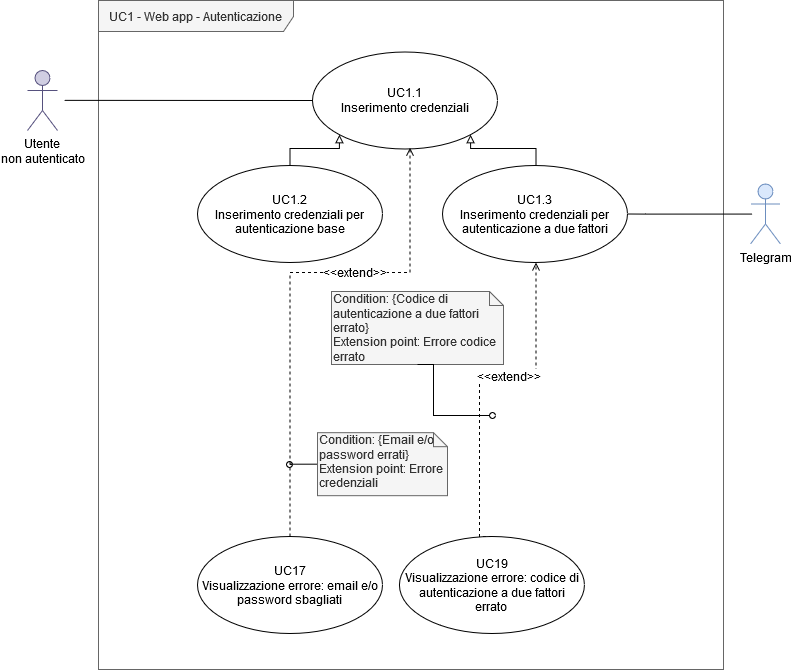
\includegraphics[height=10em]{res/images/uc1}
		%\end{figure}
		
	\begin{itemize}
		\item \textbf{Attori Primari}: Utente non autenticato.
		\item \textbf{Attori Secondari}: \glock{Telegram}.
		\item \textbf{Descrizione}: L'utente tenta di autenticarsi con il \glock{\glock{bot}} \glock{Telegram}, per farlo entra all'interno dell'applicazione e inizia la chat con il \glock{bot}. Attraverso \glock{Telegram}, viene segnalato al \glock{bot} il nome utente e il \glock{bot} verifica se questo è censito all'interno del sistema. Se viene riconosciuto, viene registrata l'apertura e l'autenticazione del canale di comunicazione tra il \glock{bot} e l'utente, diventando quest'ultimo autenticato. 
		\item \textbf{Precondizione}: L'utente è nell'applicazione di \glock{Telegram} e non ha una chat autenticata con il \glock{bot}.
		\item \textbf{Postcondizione}: L'utente effettua l'autenticazione e il canale di comunicazione tra utente e \glock{bot} viene salvato nel sistema.
		\item \textbf{Scenario Principale}:
		\begin{enumerate}
			\item L'utente seleziona nell'applicazione di \glock{Telegram} il \glock{bot} di sistema dal pannello di ricerca
			\item L'utente tenta di aprire una conversazione con il \glock{bot}
			\item L'utente viene autenticato e la chat viene salvata nel sistema
		\end{enumerate}
	\end{itemize}
	
	\subsubsection{UC 14.1 - Richiesta di riconoscimento}

	\begin{itemize}
		\item \textbf{Attori Primari}: Utente non autenticato.
		\item \textbf{Descrizione}: L'utente invia una richiesta al \glock{bot} di volersi autenticare per poter aprire il canale di comunicazione.
		\item \textbf{Precondizione}: L'utente è nell'applicazione di \glock{Telegram} e non ha una chat autenticata con il \glock{bot}.
		\item \textbf{Postcondizione}: L'utente invia il comando per richiedere l'autenticazione.
		\item \textbf{Scenario Principale}:
		\begin{enumerate}
			\item L'utente seleziona nell'applicazione di \glock{Telegram} il \glock{bot} del sistema.
			\item L'utente tenta di aprire una conversazione con il \glock{bot}.
			\item Per attivare la conversazione con il \glock{bot} ed autenticarsi, l'utente invia il comando predefinito.
		\end{enumerate}
		\item \textbf{Inclusioni}:
		\begin{itemize}
			\item Controllo credenziali (UC 14.2)
		\end{itemize}
	\end{itemize}

	\subsubsection{UC 14.2 - Controllo credenziali}

	\begin{itemize}
		\item \textbf{Attori Primari}: Utente non autenticato.
		\item \textbf{Attori Secondari}: \glock{Telegram}.
		\item \textbf{Descrizione}: Si deve verificare se il nome utente è stato censito da parte del sistema, così da abilitare la chat di comunicazione ed autenticare l'utente.
		\item \textbf{Precondizione}: L'utente, tramite \glock{Telegram}, ha inviato al \glock{bot} una richiesta di avvio conversazione con il comando predefinito.
		\item \textbf{Postcondizione}: L'utente effettua il riconoscimento con il sistema e viene autenticato.
		\item \textbf{Scenario Principale}:
		\begin{enumerate}
			\item Il \glock{Telegram} \glock{bot} riceve in input il comando che viene inoltrato al sistema, insieme alle informazioni relative alla chat e all'autore del messaggio.
			\item Viene mostrato un messaggio di benvenuto dal \glock{bot}, attraverso \glock{Telegram}, che conferma le credenziali dell'utente.
			\item L'utente viene autenticato e la chat viene salvata nel sistema.
		\end{enumerate}
		\item \textbf{Estensioni}:
		\begin{itemize}
			\item Errore: nome utente \glock{Telegram} non riconosciuto (UC 14.3)
			\item Nessuna risposta dopo una interazione con \glock{Telegram} (UC 20)
		\end{itemize}
	\end{itemize}

	\subsubsection{UC 14.3 - Errore: nome utente \glock{Telegram} non riconosciuto}

	\begin{itemize}
		\item \textbf{Attori Primari}: Utente non autenticato.
		\item \textbf{Descrizione}: L'autenticazione della chat tra il \glock{bot} e l'utente non va a buon fine dal momento che il nome utente associato all'account di \glock{Telegram} non è censito nel sistema.
		\item \textbf{Precondizione}: L'utente, tramite \glock{Telegram}, sta tentando di autenticarsi con l'invio del comando predefinito.
		\item \textbf{Postcondizione}: L'utente non viene autenticato e viene mostrato un messaggio di errore.
		\item \textbf{Scenario Principale}:
		\begin{enumerate}
			\item Il \glock{bot} \glock{Telegram} riceve in input il comando che viene inoltrato al sistema, insieme alle informazioni relative alla chat e all'autore del messaggio.
			\item Viene mostrato un messaggio di errore che segnala che il nome utente associato all'utente \glock{Telegram} non è censito nel sistema.
			\item L'utente non viene autenticato.
		\end{enumerate}
	\end{itemize}